\documentclass[12pt, a4paper]{article}

\usepackage[utf8]{inputenc}
\usepackage[T1]{fontenc}
\usepackage{geometry}
\usepackage{setspace}
\usepackage{graphicx}
\usepackage{float}
\usepackage{amsmath}
\usepackage{booktabs}
\usepackage{array}
\usepackage{xcolor}
\usepackage{hyperref}
\usepackage{charter}
\usepackage{microtype}
\usepackage{titlesec}

% Custom color used on the title page.
\definecolor{NTRA_Blue}{RGB}{0,82,155}

% Fallbacks so the document still compiles if border helpers are not loaded.
\providecommand{\MyPageBorder}{}
\providecommand{\AddToShipoutPictureFG}[1]{}

\geometry{a4paper, margin=1in}
\onehalfspacing

\titleformat{\section}{\large\bfseries}{\thesection}{1em}{}[\titlerule]
\titleformat{\subsection}{\normalsize\bfseries}{\thesubsection}{1em}{}

\begin{document}

% ==========================================
% TITLE PAGE (No Border)
% ==========================================
\begin{titlepage}
    \centering
    
    % --- Logos and Header ---
    \begin{minipage}[c]{0.2\textwidth}
        \begin{flushleft}
            
\includegraphics[width=2.5cm]{Picture1.png} 
        \end{flushleft}
    \end{minipage}%
    \hfill
    \begin{minipage}[c]{0.5\textwidth}
        \centering
        \setstretch{1.1}
        {\large \textbf{Cairo University}} \\
        {\large Faculty of Engineering} \\
        {\large Electronics \& Communications Dept.}
    \end{minipage}%
    \hfill
    \begin{minipage}[c]{0.2\textwidth}
        \begin{flushright}
            
\includegraphics[width=2.5cm]{Picture2.jpg} 
        \end{flushright}
    \end{minipage}

    \vspace{2.5cm}

    % --- Main Title ---
    \rule{\linewidth}{0.8mm} \\[0.5cm]
    {\color{NTRA_Blue} \huge \bfseries NN ASSINGMENT 1} \\[0.4cm]
    {\color{NTRA_Blue} \large ...} \\
    \rule{\linewidth}{0.8mm} \\[1.5cm]

    % \vspace{0.5cm}
    % {\large Submitted for:} \\
    % {\textbf{Dr. Mohsen Ra}}

    \vfill

    % --- Team and Professor Info ---
    \begin{center}
        \setstretch{1.5}
        \textbf{Prepared by:} \\[0.3cm]
        \begin{tabular}{l r}
        \textbf{Abdallah Essam Mohamed Mahmoud} & \hspace{1cm} ID: ... \\
            \textbf{Zeyad Antar Othman Abu-Zaid} & \hspace{1cm} ID: 9220331 \\
            \textbf{Abdelrahman Hatem} & \hspace{1cm} ID: ... \\            
            \end{tabular}

        \vspace{1cm}

        \textbf{Submitted to:} \\
        \textbf{Dr. Fadel Dighm} \\
    \end{center}

    \vfill
    \rule{0.3\linewidth}{0.2mm} \\
    {\large February 2026}
\end{titlepage}

% --- ACTIVATE BORDER AFTER TITLE PAGE ---
\AddToShipoutPictureFG{\MyPageBorder} 


\tableofcontents
\newpage

\section{Part 1}
Part 1 is documented separately.

\section{Part 2: Classical ML Modeling}

\subsection{Problem Summary and Required Tasks}
ReducedMNIST is used with 10 classes (digits 0--9), where the training split has 1000 samples per class and the testing split has 200 samples per class.

The required tasks are:
\begin{enumerate}
    \item Extract three feature families for train and test sets:
    \begin{itemize}
        \item DCT with 225 dimensions,
        \item PCA with cumulative variance at least 95\%,
        \item HOG features.
    \end{itemize}
    \item Train and evaluate:
    \begin{itemize}
        \item K-means per class with \(K = 1, 4, 16, 32\),
        \item SVM with linear and nonlinear kernels.
    \end{itemize}
    \item Report comparative accuracy and processing time in one final table.
    \item Show confusion matrices only for the best K-means result and the best SVM result.
    \item Add conclusions.
\end{enumerate}

\subsection{Implementation Flow}
The implemented flow in Part\_2 scripts is:
\begin{enumerate}
    \item Load ReducedMNIST (JPG folder dataset via KaggleHub, with safe fallbacks).
    \item Normalize pixel values to \([0,1]\).
    \item Extract DCT, PCA, and HOG features.
    \item Train K-means per class for \(K \in \{1,4,16,32\}\) and evaluate on test data.
    \item Train SVM with linear and RBF kernels and evaluate on test data.
    \item Store predictions, measure real elapsed time, and print summary tables.
    \item Visualize confusion matrices and comparative charts.
\end{enumerate}

\subsection{Nonlinear SVM Used (RBF) and Its Specifications}
The nonlinear model used in this implementation is \textbf{C-SVC with RBF kernel} from scikit-learn.

The kernel function is:
\[
K(\mathbf{x},\mathbf{z}) = \exp\left(-\gamma\lVert \mathbf{x}-\mathbf{z} \rVert^2\right)
\]
which enables curved (nonlinear) decision boundaries for classes that are not linearly separable.

Exact settings used in code (Part\_2/step3\_svm.py):
\begin{itemize}
    \item \texttt{kernel='rbf'}
    \item \(C = 10.0\)
    \item \(\gamma = \texttt{scale}\)
    \item \texttt{decision\_function\_shape='ovo'} (one-vs-one multiclass)
\end{itemize}

Feature scaling step before SVM training/inference:
\begin{itemize}
    \item \texttt{StandardScaler()} is fitted on training features.
    \item The same scaler is applied to both train and test features.
\end{itemize}

For \(\gamma = \texttt{scale}\), scikit-learn uses:
\[
\gamma = \frac{1}{n_{\text{features}}\,\mathrm{Var}(X)}
\]
All remaining \texttt{SVC} parameters are left at library defaults.

\subsection{Comparative Results (Accuracy and Processing Time)}
Table~\ref{tab:part2_results} summarizes all required combinations with measured real elapsed time.

\begin{table}[H]
\centering
\small
\setlength{\tabcolsep}{5pt}
\begin{tabular}{l|cc|cc|cc}
\toprule
\textbf{Classifier} & \multicolumn{2}{c|}{\textbf{DCT}} & \multicolumn{2}{c|}{\textbf{PCA}} & \multicolumn{2}{c}{\textbf{HOG}} \\
 & Acc. (\%) & Time (s) & Acc. (\%) & Time (s) & Acc. (\%) & Time (s) \\
\midrule
K-means \(K=1\)  & 86.85 & 0.01 & 86.80 & 0.00 & 91.35 & 0.04 \\
K-means \(K=4\)  & 92.65 & 2.19 & 92.30 & 0.61 & 93.60 & 8.00 \\
K-means \(K=16\) & 94.85 & 1.50 & 94.80 & 1.51 & 95.00 & 17.85 \\
K-means \(K=32\) & 96.15 & 2.05 & 95.70 & 2.14 & 96.00 & 29.79 \\
SVM Linear         & 92.60 & 1.78 & 90.65 & 2.66 & 96.70 & 10.80 \\
SVM Nonlinear (RBF, \(C=10\), \(\gamma=\)scale) & 96.90 & 5.05 & 95.40 & 12.54 & 96.70 & 31.02 \\
\bottomrule
\end{tabular}
\caption{Part 2 required comparative table: accuracy and processing time.}
\label{tab:part2_results}
\end{table}

\subsection{Best Results and Confusion Matrices}
Best K-means result: \textbf{K-means \(K=32\) with DCT} (96.15\%).\\
Best SVM result: \textbf{SVM Nonlinear (RBF) with DCT} (96.90\%).

\begin{figure}[H]
\centering
\IfFileExists{Part_2/figures/cm_kmeans_best.png}{
    \includegraphics[width=0.62\textwidth]{Part_2/figures/cm_kmeans_best.png}
}{
    \fbox{\parbox{0.85\textwidth}{Insert confusion matrix image for best K-means result here (K=32 with DCT).}}
}
\caption{Confusion matrix for the best K-means model.}
\end{figure}

\begin{figure}[H]
\centering
\IfFileExists{PART2_screenshorts/ALL_PLOTS.png}{
    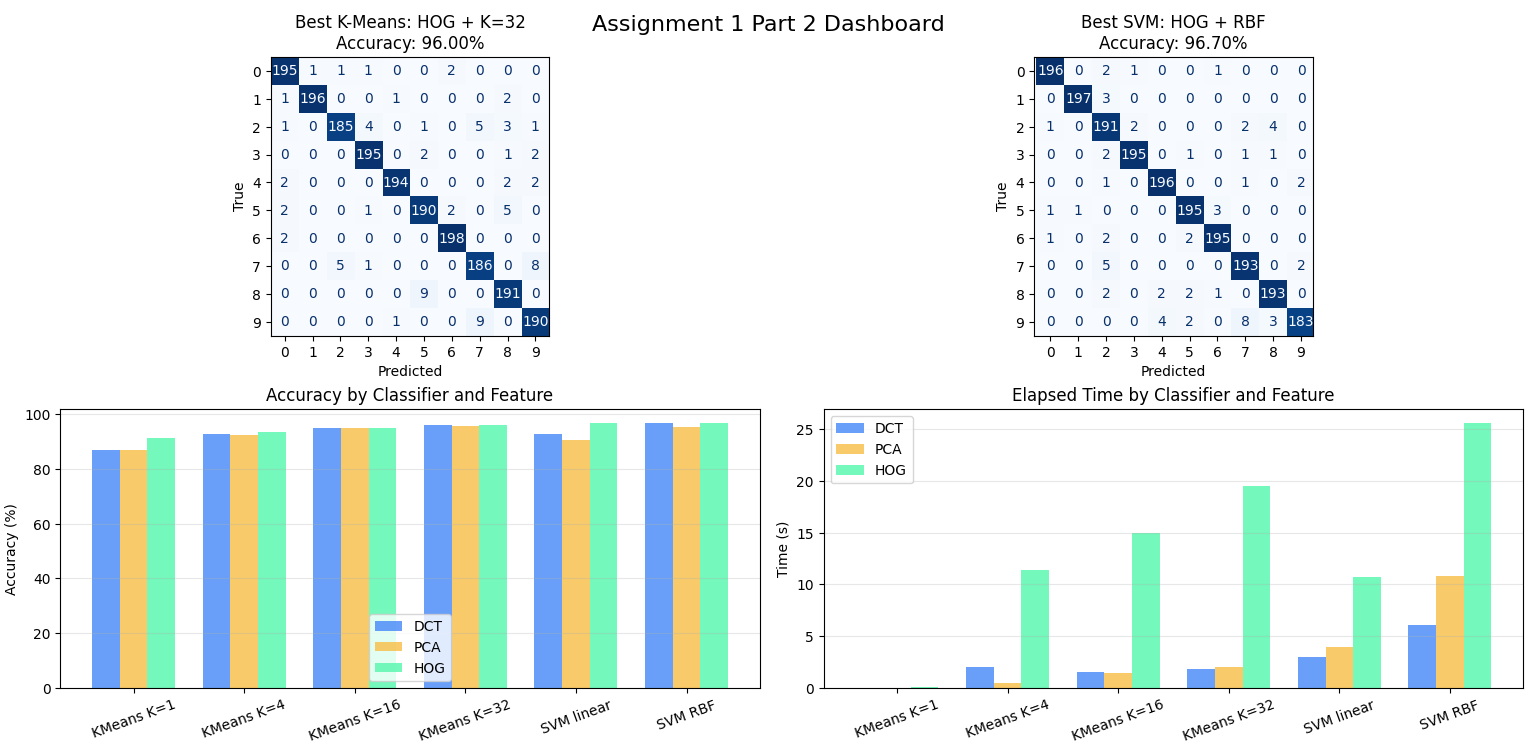
\includegraphics[width=0.62\textwidth]{PART2_screenshorts/ALL_PLOTS.png}
}{
    \fbox{\parbox{0.85\textwidth}{Insert confusion matrix image for best SVM result here (RBF with DCT).}}
}
\caption{Confusion matrix for the best SVM model.}
\end{figure}

\subsection{Conclusions}
\begin{enumerate}
    \item Increasing \(K\) in class-wise K-means consistently improves performance, with best result at \(K=32\).
    \item Nonlinear SVM (RBF) gives the highest overall accuracy among all tested combinations.
    \item HOG is competitive, especially for linear SVM, but incurs higher runtime.
    \item DCT features produced the strongest best-case accuracy for both classifier families in this run.
    \item Reporting both accuracy and elapsed time is important because the best-accuracy model is not always the fastest one.
\end{enumerate}

\end{document}
